\documentclass[zihao=5,a4paper,UTF8]{ctexart}
\usepackage[top=2.0cm, bottom=2.0cm, left=2.0cm, right=2.0cm]{geometry}
\usepackage{amsmath, amssymb, bm}
\newcommand{\vect}[1]{\bm{#1}}
\newcommand{\ee}{\mathrm{e}}
\usepackage{array, booktabs}
\usepackage{enumitem}
\usepackage{tikz}
\usepackage{fancyhdr}

\pagestyle{fancy}
\fancyhf{}
\fancyfoot[C]{\small 第 \thepage\ 页}
\renewcommand{\headrulewidth}{0pt}

\newcommand{\blank}[1][2.5cm]{\underline{\hspace{#1}}}
\newcommand{\choicebox}{\hfill(\hspace{1.8em})}

\begin{document}

\begin{center}
    {\Large\bfseries 南京航空航天大学}\\[4pt]
    {\large 2021 $\sim$ 2022 学年\ 第 1 学期\ 《大学物理 I(2)》、《大学物理 IA(2)》考试试题}
\end{center}

\begin{center}
\begin{tabular}{|c|c|c|c|c|}
\hline
题号 & 一（36分） & 二（30分） & 三（34分） & 总分 \\
\hline
得分 & \hspace{2.2cm} & \hspace{2.2cm} & \hspace{2.2cm} & \hspace{2.2cm} \\
\hline
\end{tabular}
\end{center}

\section*{一、选择题（每小题 3 分，共 36 分）}

\begin{enumerate}[leftmargin=2em, itemsep=6pt]
    \item 一个质点作简谐运动，振幅为 $A$，在起始时刻质点的位移为 $-A/2$，且向 $x$ 轴正方向运动，代表此简谐运动的旋转矢量图为：\choicebox\\
    \begin{center}
    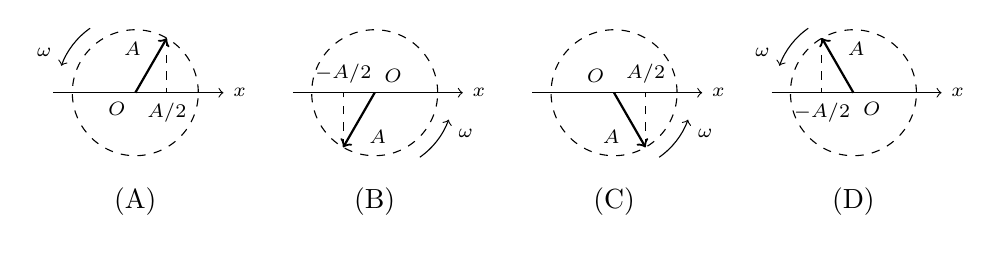
\begin{tikzpicture}[scale=0.80]
        % (A)
        \begin{scope}
            \draw[dashed] (0,0) circle (1);
            \draw[->] (-1.3,0) -- (1.4,0) node[right] {\scriptsize $x$};
            \draw[->, thick] (0,0) -- (60:1) node[midway, above left] {\scriptsize $A$};
            \draw[dashed] (60:1) -- (0.5,0) node[below] {\scriptsize $A/2$};
            \node[below left] at (0,0) {\scriptsize $O$};
            \draw[->] (125:1.25) arc (125:160:1.25) node[above left] {\scriptsize $\omega$};
            \node[below] at (0,-1.35) {(A)};
        \end{scope}
        % (B)
        \begin{scope}[xshift=3.8cm]
            \draw[dashed] (0,0) circle (1);
            \draw[->] (-1.3,0) -- (1.4,0) node[right] {\scriptsize $x$};
            \draw[->, thick] (0,0) -- (-120:1) node[midway, below right] {\scriptsize $A$};
            \draw[dashed] (-120:1) -- (-0.5,0) node[above] {\scriptsize $-A/2$};
            \node[above right] at (0,0) {\scriptsize $O$};
            \draw[->] (-55:1.25) arc (-55:-20:1.25) node[below right] {\scriptsize $\omega$};
            \node[below] at (0,-1.35) {(B)};
        \end{scope}
        % (C)
        \begin{scope}[xshift=7.6cm]
            \draw[dashed] (0,0) circle (1);
            \draw[->] (-1.3,0) -- (1.4,0) node[right] {\scriptsize $x$};
            \draw[->, thick] (0,0) -- (-60:1) node[midway, below left] {\scriptsize $A$};
            \draw[dashed] (-60:1) -- (0.5,0) node[above] {\scriptsize $A/2$};
            \node[above left] at (0,0) {\scriptsize $O$};
            \draw[->] (-55:1.25) arc (-55:-20:1.25) node[below right] {\scriptsize $\omega$};
            \node[below] at (0,-1.35) {(C)};
        \end{scope}
        % (D)
        \begin{scope}[xshift=11.4cm]
            \draw[dashed] (0,0) circle (1);
            \draw[->] (-1.3,0) -- (1.4,0) node[right] {\scriptsize $x$};
            \draw[->, thick] (0,0) -- (120:1) node[midway, above right] {\scriptsize $A$};
            \draw[dashed] (120:1) -- (-0.5,0) node[below] {\scriptsize $-A/2$};
            \node[below right] at (0,0) {\scriptsize $O$};
            \draw[->] (125:1.25) arc (125:160:1.25) node[above left] {\scriptsize $\omega$};
            \node[below] at (0,-1.35) {(D)};
        \end{scope}
    \end{tikzpicture}
    \end{center}

    \item 一简谐振动曲线如图所示（$t=0$ 时 $x=2\ \mathrm{cm}$ 且斜率为正，振幅 $A=4\ \mathrm{cm}$，$t=1\ \mathrm{s}$ 时首次从上方穿过 $x=0$），则振动周期为\choicebox\\
    \begin{minipage}[t]{0.68\textwidth}
    (A) $2.62\ \mathrm{s}$\qquad (B) $2.40\ \mathrm{s}$\qquad (C) $2.20\ \mathrm{s}$\qquad (D) $2.00\ \mathrm{s}$
    \end{minipage}%
    \begin{minipage}[t]{0.30\textwidth}
    \centering
    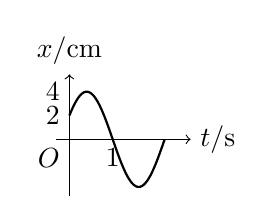
\begin{tikzpicture}[scale=0.55, baseline=(current bounding box.north)]
        \draw[->] (-0.3,0) -- (2.8,0) node[right] {$t/\mathrm{s}$};
        \draw[->] (0,-1.3) -- (0,1.5) node[above] {$x/\mathrm{cm}$};
        \draw[thick, domain=0:2.2, samples=60] plot (\x, {1.1*cos(150*\x - 60)});
        \node[below left] at (0,0) {$O$};
        \node[left] at (0,0.55) {$2$};
        \node[left] at (0,1.1) {$4$};
        \node[below] at (1.0,0) {$1$};
    \end{tikzpicture}
    \end{minipage}

    \item 下图（a）表示沿 $x$ 轴正向传播的平面简谐波在 $t=0$ 时刻的波形图，则图（b）表示的是\choicebox\\
    \begin{minipage}[t]{0.46\textwidth}
    (A) 质点 $m$ 的振动曲线；\qquad (B) 质点 $n$ 的振动曲线；\\
    (C) 质点 $p$ 的振动曲线；\qquad (D) 质点 $q$ 的振动曲线。
    \end{minipage}%
    \begin{minipage}[t]{0.52\textwidth}
    \centering
    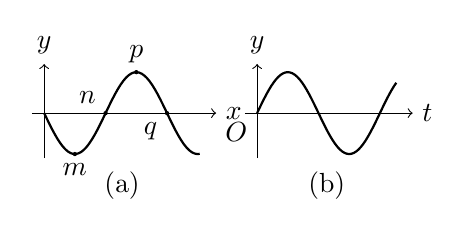
\begin{tikzpicture}[scale=0.52, baseline=(current bounding box.north)]
        % (a)
        \draw[->] (-0.3,0) -- (4.2,0) node[right] {$x$};
        \draw[->] (0,-1.1) -- (0,1.2) node[above] {$y$};
        \draw[thick, domain=0:3.8, samples=60] plot (\x, {-sin(120*\x)});
        \fill (0.75,-1) circle (1.5pt) node[below] {$m$};
        \fill (1.5,0) circle (1.5pt) node[above left] {$n$};
        \fill (2.25,1) circle (1.5pt) node[above] {$p$};
        \fill (3.0,0) circle (1.5pt) node[below left] {$q$};
        \node[below] at (1.9,-1.2) {(a)};
        % (b)
        \begin{scope}[xshift=5.2cm]
            \draw[->] (-0.3,0) -- (3.8,0) node[right] {$t$};
            \draw[->] (0,-1.1) -- (0,1.2) node[above] {$y$};
            \draw[thick, domain=0:3.4, samples=60] plot (\x, {sin(120*\x)});
            \node[below left] at (0,0) {$O$};
            \node[below] at (1.7,-1.2) {(b)};
        \end{scope}
    \end{tikzpicture}
    \end{minipage}

    \item 某时刻驻波波形曲线如图所示，则 $a$、$b$ 两点振动的相位差是\choicebox\\
    \begin{minipage}[t]{0.65\textwidth}
    (A) $0$\qquad (B) $\frac{1}{2}\pi$\qquad (C) $\pi$\qquad (D) $5\pi/4$
    \end{minipage}%
    \begin{minipage}[t]{0.33\textwidth}
    \centering
    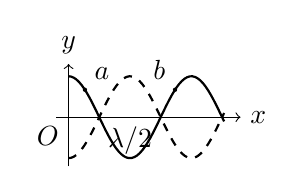
\begin{tikzpicture}[scale=0.52, baseline=(current bounding box.north)]
        \draw[->] (-0.3,0) -- (4.2,0) node[right] {$x$};
        \draw[->] (0,-1.2) -- (0,1.3) node[above] {$y$};
        \draw[thick, domain=0:3.8, samples=60] plot (\x, {cos(120*\x)});
        \draw[thick, dashed, domain=0:3.8, samples=60] plot (\x, {-cos(120*\x)});
        \fill (0.4,0.67) circle (1.5pt) node[above right] {$a$};
        \fill (2.6,0.67) circle (1.5pt) node[above left] {$b$};
        \node[below] at (1.5,0) {$\lambda/2$};
        \node[below left] at (0,0) {$O$};
    \end{tikzpicture}
    \end{minipage}

    \item 在照相机镜头的玻璃上均匀镀有一层介质薄膜，其折射率 $n$ 小于玻璃的折射率。假定光线垂直照射镜头，要使得某一波长 $\lambda$ 透射光增强，则介质膜的最小厚度应为\choicebox\\
    (A) $\frac{\lambda}{n}$\qquad (B) $\frac{\lambda}{2n}$\qquad (C) $\frac{\lambda}{3n}$\qquad (D) $\frac{\lambda}{4n}$

    \item \begin{minipage}[t]{0.64\textwidth}
    在如图所示的单缝夫琅禾费衍射实验中，若将单缝沿透镜光轴方向向透镜平移，则屏幕上的衍射条纹\choicebox\\
    (A) 间距变大；\qquad\qquad (B) 间距变小；\\
    (C) 不发生变化；\qquad\quad (D) 间距不变，但明暗条纹的位置交替变化。
    \end{minipage}%
    \begin{minipage}[t]{0.34\textwidth}
    \centering
    \begin{tikzpicture}[scale=0.62, baseline=(current bounding box.north)]
        \draw[very thick] (0,1.1) -- (0,0.35);
        \draw[very thick] (0,-0.35) -- (0,-1.1);
        \node[above] at (0,1.1) {\scriptsize 单缝};
        \draw[dashed] (-0.8,0) -- (2.8,0);
        \draw[->, >=stealth] (-0.9,0.25) -- (0,0.25);
        \draw[->, >=stealth] (-0.9,-0.25) -- (0,-0.25);
        \node[left] at (-0.9,0.25) {\scriptsize $\lambda$};
        \draw[thick] (1.1,-1.0) .. controls (1.35,-0.3) and (1.35,0.3) .. (1.1,1.0);
        \draw[thick] (1.1,-1.0) .. controls (0.85,-0.3) and (0.85,0.3) .. (1.1,1.0);
        \node[above] at (1.1,1.05) {\scriptsize $L$};
        \draw[thick] (2.8,-1.1) -- (2.8,1.1);
        \node[above] at (2.8,1.1) {\scriptsize 屏幕};
        \draw[<->, >=stealth, thin] (1.1,-1.15) -- (2.8,-1.15) node[midway, below] {\scriptsize $f$};
    \end{tikzpicture}
    \end{minipage}

    \item 波长 $\lambda$ 为 $600\ \mathrm{nm}$ 的单色光垂直入射到光栅常数为 $2.5\times 10^{-3}\ \mathrm{mm}$ 的光栅上，光栅的不透光宽与透光狭缝宽相等，则光谱上呈现的全部级数为\choicebox\\
    (A) $0, \pm 1, \pm 2, \pm 3, \pm 4$\qquad (B) $0, \pm 1, \pm 3$\qquad (C) $\pm 1, \pm 3$\qquad (D) $0, \pm 2, \pm 4$

    \item 使光强为 $I_0$ 的平面偏振光先后通过两个偏振片 $P_1$ 和 $P_2$，$P_1$ 和 $P_2$ 的偏振化方向与原入射光矢量振动方向的夹角分别是 $\alpha$ 和 $90^\circ$，则通过这两个偏振片后的光强 $I$ 是\choicebox\\
    (A) $\frac{1}{2}I_0\cos^2\alpha$\qquad (B) $0$\qquad (C) $\frac{1}{4}I_0\sin^2(2\alpha)$\qquad (D) $\frac{1}{4}I_0\sin^2\alpha$

    \item 波长 $\lambda=5000\ \text{\AA}$ 的光波沿 $x$ 轴正向传播，若光的波长的不确定量 $\Delta\lambda = 10^{-3}\ \text{\AA}$，则利用不确定关系 $\Delta p_x \Delta x \ge h$ 可得光子的 $x$ 坐标的不确定量至少为：\choicebox\\
    (A) $25\ \mathrm{cm}$\qquad (B) $50\ \mathrm{cm}$\qquad (C) $250\ \mathrm{cm}$\qquad (D) $500\ \mathrm{cm}$

    \item 已知粒子处于宽度为 $a$ 的一维无限深势阱中运动的波函数为 $\psi_n(x) = \sqrt{\frac{2}{a}}\sin\frac{n\pi x}{a}\ (n=1,2,3,\dots)$，则当 $n=1$ 基态时，在 $x_1=0 \to x_2=a/3$ 区间找到粒子的概率为\choicebox\\
    (A) $0.09$\qquad (B) $0.19$\qquad (C) $0.33$\qquad (D) $0.81$

    \item 用频率为 $\nu_1$ 的单色光照射某种金属时，测得饱和电流为 $I_1$，以频率为 $\nu_2$ 的单色光照射该金属时，测得饱和电流为 $I_2$，若 $I_1 > I_2$，则\choicebox\\
    (A) $\nu_1 > \nu_2$\qquad (B) $\nu_1 < \nu_2$\qquad (C) $\nu_1 = \nu_2$\qquad (D) $\nu_1$ 与 $\nu_2$ 的关系还不能确定

    \item 某金属产生光电效应的红限频率为 $\nu_0$，当用频率为 $\nu\ (\nu > \nu_0)$ 的单色光照射该金属时，从金属中逸出的光电子（质量为 $m$）的德布罗意波长为\choicebox\\
    (A) $\sqrt{\frac{h}{2m(\nu+\nu_0)}}$\qquad (B) $\sqrt{\frac{h}{2m(\nu-\nu_0)}}$\qquad (C) $\sqrt{\frac{h\nu_0}{2m\nu}}$\qquad (D) $\sqrt{\frac{2h}{m(\nu-\nu_0)}}$
\end{enumerate}

\section*{二、填空题（每空 3 分，共 30 分）}

\begin{enumerate}[leftmargin=2em, itemsep=6pt, start=13]
    \item 原长为 $0.5\ \mathrm{m}$ 的弹簧，上端固定，下端挂一质量为 $0.1\ \mathrm{kg}$ 的物体，当物体静止时，弹簧长为 $0.6\ \mathrm{m}$。现将物体上推，使弹簧缩回到原长，然后放手，以放手时开始计时，取竖直向下为正向，写出振动表达式\blank[4.5cm]。

    \item 图中所示为两个简谐振动的振动曲线，若以余弦函数表示这两个振动的合成结果，则合振动的方程为 $x = x_1 + x_2 = \blank[4.0cm]$。
    \begin{center}
    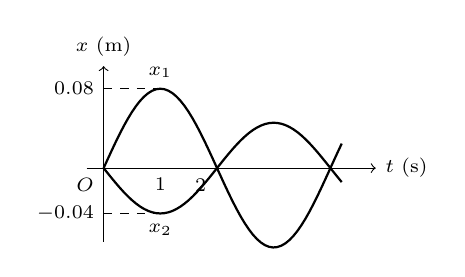
\begin{tikzpicture}[scale=0.72]
        \draw[->] (-0.3,0) -- (4.8,0) node[right] {\scriptsize $t\ (\mathrm{s})$};
        \draw[->] (0,-1.3) -- (0,1.8) node[above] {\scriptsize $x\ (\mathrm{m})$};
        \draw[thick, domain=0:4.2, samples=60] plot (\x, {-0.8*sin(90*\x)});
        \draw[thick, domain=0:4.2, samples=60] plot (\x, {1.4*sin(90*\x)});
        \draw[dashed] (0,1.4) node[left] {\scriptsize $0.08$} -- (1,1.4);
        \draw[dashed] (0,-0.8) node[left] {\scriptsize $-0.04$} -- (1,-0.8);
        \node[below left] at (0,0) {\scriptsize $O$};
        \node[below] at (1,0) {\scriptsize $1$};
        \node[below left] at (1.98,-0.02) {\scriptsize $2$};
        \node[above] at (1.0,1.42) {\scriptsize $x_1$};
        \node[below] at (1.0,-0.82) {\scriptsize $x_2$};
    \end{tikzpicture}
    \end{center}

    \item 有两艘潜艇在水中相向而行，甲的速度为 $50.0\ \mathrm{km\cdot h^{-1}}$，乙的速度为 $70\ \mathrm{km\cdot h^{-1}}$，如图所示，甲潜艇发出一个 $1.0\times 10^3\ \mathrm{Hz}$ 的声音信号，设声波在水中的传播速度为 $5.47\times 10^3\ \mathrm{km\cdot h^{-1}}$，则甲潜艇接收到的从乙潜艇反射回来的信号频率\blank[2.8cm]。
    \begin{center}
    \begin{tikzpicture}[scale=0.7]
        % 潜艇甲 (左)
        \draw[thick, rounded corners=6pt] (-3.2,-0.22) rectangle (-1.5,0.22);
        \draw[thick] (-2.6,0.22) -- (-2.6,0.45) -- (-2.2,0.45) -- (-2.2,0.22);
        \draw[thick] (-3.2,-0.15) -- (-3.45,-0.25) -- (-3.45,0.25) -- (-3.2,0.15);
        \draw[->, >=stealth] (-2.8,-0.4) -- (-1.9,-0.4);
        \node[below] at (-2.35,-0.45) {\scriptsize 甲 $50.0\ \mathrm{km\cdot h^{-1}}$};
        % 声波波面
        \foreach \x in {-1.2,-0.9,-0.6,-0.3,0.0} {\draw (\x+0.15,0.2) arc (30:-30:0.4);}
        \foreach \x in {0.3,0.6,0.9,1.2} {\draw (\x,-0.2) arc (210:150:0.4);}
        % 潜艇乙 (右)
        \draw[thick, rounded corners=6pt] (1.5,-0.22) rectangle (3.2,0.22);
        \draw[thick] (2.2,0.22) -- (2.2,0.45) -- (2.6,0.45) -- (2.6,0.22);
        \draw[thick] (3.2,-0.15) -- (3.45,-0.25) -- (3.45,0.25) -- (3.2,0.15);
        \draw[->, >=stealth] (2.8,-0.4) -- (1.9,-0.4);
        \node[below] at (2.35,-0.45) {\scriptsize 乙 $70.0\ \mathrm{km\cdot h^{-1}}$};
    \end{tikzpicture}
    \end{center}

    \item 设入射波的表达式为 $y_1 = A\cos\left[2\pi\left(\nu t + \frac{x}{\lambda}\right) + \pi\right]$，波在 $x=0$ 处发生反射，反射点为一固定端，则入射波和反射波合成驻波的波腹坐标为\blank[3.5cm]。

    \item 在单缝夫琅禾费衍射实验中波长为 $\lambda$ 的单色光垂直入射在宽度为 $a=2\lambda$ 的单缝上，对应于衍射角为 $30^\circ$ 方向，单缝处的波面可分成的半波带数目为\blank[2.0cm]个。

    \item 设白天人的眼瞳直径为 $3\ \mathrm{mm}$，入射光波长为 $550\ \mathrm{nm}$，窗纱上两根细丝之间的距离为 $3\ \mathrm{mm}$，人眼睛可以距离窗纱\blank[2.2cm]$\mathrm{m}$ 时，恰能分辨。

    \item 测量不透明介质折射率的一种方法是，用一束自然光从真空入射介质表面，当反射光为线偏振光时，测得此时的反射角为 $60^\circ$，则介质的折射率为\blank[2.2cm]。

    \item 对黑体加热后，测得总的辐出度（即单位面积辐射功率）增大为原来的 $16$ 倍，则黑体的温度为原来的\blank[2.0cm]倍。

    \item 可用光电效应测定普朗克常数。如先后分别用波长 $\lambda_1$ 和 $\lambda_2$ 做光电效应实验，相应测得其遏止电势差为 $U_1$ 和 $U_2$，则可算得普朗克常数\blank[4.0cm]。

    \item \begin{minipage}[t]{0.68\textwidth}
    如图所示，频率为 $\nu$ 的入射光子与静止的自由电子发生碰撞和散射。如果散射光子的频率为 $\nu'$，反冲电子的动量为 $\vect{p}$，则在入射光子方向上的动量守恒定律的分量式为\blank[4.5cm]。
    \end{minipage}%
    \begin{minipage}[t]{0.30\textwidth}
    \centering
    \begin{tikzpicture}[scale=0.68, baseline=(current bounding box.north)]
        \draw[->, >=stealth, thick] (-1.4,0) -- (0,0) node[midway, above] {\scriptsize $\nu$};
        \draw[dashed] (0,0) -- (1.6,0);
        \draw[->, >=stealth, thick] (0,0) -- (40:1.4) node[above] {\scriptsize $\nu'$};
        \draw[->, >=stealth, thick] (0,0) -- (-42:1.4) node[below] {\scriptsize $e\text{ 反冲电子}$};
        \draw (0.55,0) arc (0:40:0.55);
        \node at (0.78,0.25) {\scriptsize $\phi$};
        \draw (0.5,0) arc (0:-42:0.5);
        \node at (0.72,-0.25) {\scriptsize $\theta$};
    \end{tikzpicture}
    \end{minipage}
\end{enumerate}

\section*{三、计算题（共 34 分）}

\begin{enumerate}[leftmargin=2em, itemsep=8pt, start=23]
    \item （10 分）如图所示，为一沿 $x$ 轴正向传播的平面简谐波在 $t=1/3\ \mathrm{s}$ 时的波形，其周期 $T=2\ \mathrm{s}$。求：\\
    （1）$O$ 点和 $P$ 点的振动表达式；\\
    （2）波函数；\\
    （3）$P$ 点离 $O$ 点的距离。
    \begin{center}
    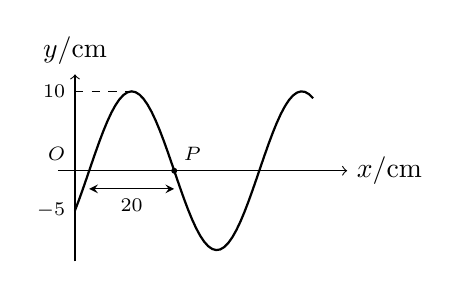
\begin{tikzpicture}[scale=0.72]
        \draw[->] (-0.3,0) -- (4.8,0) node[right] {$x/\mathrm{cm}$};
        \draw[->] (0,-1.6) -- (0,1.7) node[above] {$y/\mathrm{cm}$};
        \draw[thick, domain=0:4.2, samples=60] plot (\x, {1.4*sin(120*\x - 30)});
        \draw[dashed] (0,1.4) node[left] {\scriptsize $10$} -- (1.0,1.4);
        \node[left] at (0,-0.7) {\scriptsize $-5$};
        \node[above left] at (0,0) {\scriptsize $O$};
        \fill (1.75,0) circle (1.5pt) node[above right] {\scriptsize $P$};
        \draw[<->, >=stealth] (0.25,-0.32) -- (1.75,-0.32) node[midway, below] {\scriptsize $20$};
    \end{tikzpicture}
    \end{center}

    \item \begin{minipage}[t]{0.68\textwidth}
    （6 分）在图示的双缝干涉实验中，若用薄玻璃片（折射率 $n_1=1.4$）覆盖缝 $S_1$，用同样厚度的玻璃片（但折射率 $n_2=1.7$）覆盖缝 $S_2$，将使原来未放玻璃时屏上的中央明条纹处 $O$ 变为第五级明纹。设单色光波长 $\lambda=480\ \mathrm{nm}$，求玻璃片的厚度 $d$（可认为光线垂直穿过玻璃片）。
    \end{minipage}%
    \begin{minipage}[t]{0.30\textwidth}
    \centering
    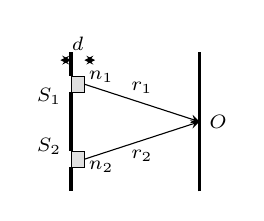
\begin{tikzpicture}[scale=0.68, baseline=(current bounding box.north)]
        % 挡板与双缝
        \draw[very thick] (0,1.3) -- (0,0.85);
        \draw[very thick] (0,0.55) -- (0,-0.55);
        \draw[very thick] (0,-0.85) -- (0,-1.3);
        % 玻璃片
        \draw[fill=gray!25] (0,0.55) rectangle (0.25,0.85);
        \draw[fill=gray!25] (0,-0.85) rectangle (0.25,-0.55);
        \node[below left] at (0,0.8) {\scriptsize $S_1$};
        \node[above left] at (0,-0.8) {\scriptsize $S_2$};
        \node[above right] at (0.15,0.55) {\scriptsize $n_1$};
        \node[below right] at (0.15,-0.55) {\scriptsize $n_2$};
        % 厚度 d
        \draw[<->, >=stealth, thin] (-0.2,1.15) -- (0,1.15);
        \draw[<->, >=stealth, thin] (0.45,1.15) -- (0.25,1.15);
        \node[above] at (0.125,1.15) {\scriptsize $d$};
        % 光屏与光线
        \draw[thick] (2.4,-1.3) -- (2.4,1.3);
        \draw[->, >=stealth] (0.25,0.7) -- (2.4,0) node[midway, above] {\scriptsize $r_1$};
        \draw[->, >=stealth] (0.25,-0.7) -- (2.4,0) node[midway, below] {\scriptsize $r_2$};
        \node[right] at (2.4,0) {\scriptsize $O$};
    \end{tikzpicture}
    \end{minipage}

    \item （10 分）一束平行光垂直入射到光栅上，该光束有两种波长的光，$\lambda_1 = 440\ \mathrm{nm}$，$\lambda_2 = 660\ \mathrm{nm}$。实验发现，两种波长的谱线（不计中央明纹）第二次重合于衍射角 $\varphi=60^\circ$ 的方向上，求此光栅的光栅常数 $d$。

    \item \begin{minipage}[t]{0.62\textwidth}
    （8 分）柱面平凹透镜 $A$，曲率半径为 $R$，放在平玻璃片 $B$ 上，如图所示。现用波长为 $\lambda$ 的平行单色光自上方垂直往下照射，观察 $A$ 和 $B$ 间空气薄膜的反射光的干涉条纹。设空气膜的最大厚度 $d=2\lambda$，求：\\
    （1）图中的 $r$ 满足什么条件时形成明条纹；\\
    （2）共能看到多少条明条纹；\\
    （3）若将玻璃片 $B$ 向下平移，条纹如何移动。
    \end{minipage}%
    \begin{minipage}[t]{0.36\textwidth}
    \centering
    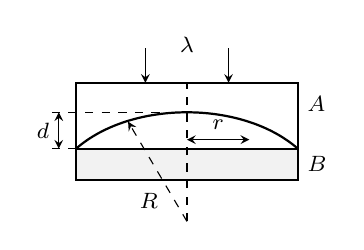
\begin{tikzpicture}[scale=0.88, baseline=(current bounding box.north)]
        % 平玻璃片 B
        \draw[thick, fill=gray!10] (-1.6,-0.45) rectangle (1.6,0);
        \node[right] at (1.6,-0.22) {\footnotesize $B$};
        % 柱面平凹透镜 A
        \draw[thick] (-1.6,0) -- (-1.6,0.95) -- (1.6,0.95) -- (1.6,0);
        \draw[thick] (-1.6,0) .. controls (-0.8,0.7) and (0.8,0.7) .. (1.6,0);
        \node[right] at (1.6,0.65) {\footnotesize $A$};
        % 垂直光线
        \draw[->, >=stealth] (-0.6,1.45) -- (-0.6,0.95);
        \draw[->, >=stealth] (0.6,1.45) -- (0.6,0.95);
        \node[above] at (0,1.25) {\footnotesize $\lambda$};
        % 中心竖直虚线
        \draw[dashed, thin] (0,-1.05) -- (0,0.95);
        % 最大厚度 d (标在左侧外部)
        \draw[dashed, thin] (-1.95,0.525) -- (0,0.525);
        \draw[dashed, thin] (-1.95,0) -- (-1.6,0);
        \draw[<->, >=stealth, thin] (-1.85,0) -- (-1.85,0.525) node[midway, left] {\footnotesize $d$};
        % 水平距离 r (标在右侧)
        \draw[<->, >=stealth, thin] (0,0.13) -- (0.9,0.13) node[midway, above] {\footnotesize $r$};
        % 曲率半径 R (从下方曲率中心指向左侧弧面，完全避开 r)
        \draw[->, >=stealth, dashed, thin] (0,-1.05) -- (-0.85,0.39);
        \node[left] at (-0.28,-0.75) {\footnotesize $R$};
    \end{tikzpicture}
    \end{minipage}
\end{enumerate}

\end{document}
